%% ============================================================
%% Research idea note (2 pages)
%% From Molecular Descriptors to Plant Performance:
%% A Geostatistical Learning Framework for Flotation Reagent Design
%% ============================================================
\documentclass[10pt]{article}

\usepackage[a4paper,margin=1.7cm,top=1.4cm,bottom=1.4cm]{geometry}
\usepackage{amsmath}
\usepackage{amssymb}
\usepackage{graphicx}
\graphicspath{{figure/}}
\usepackage[hidelinks]{hyperref}
\usepackage{microtype}
\usepackage{caption}
\usepackage{titlesec}

\captionsetup{font=small,skip=4pt}
\titlespacing*{\section}{0pt}{7pt}{2pt}
\titleformat{\section}{\normalfont\large\bfseries}{\thesection}{0.6em}{}

\setlength{\parskip}{2pt}
\setlength{\abovedisplayskip}{4pt}
\setlength{\belowdisplayskip}{4pt}

\renewcommand{\topfraction}{0.94}
\renewcommand{\bottomfraction}{0.88}
\renewcommand{\textfraction}{0.05}
\renewcommand{\floatpagefraction}{0.88}

\begin{document}

\begin{center}
{\large\bfseries From Molecular Descriptors to Plant Performance}\\[2pt]
{\bfseries A Geostatistical Learning Framework for Flotation Reagent Design}\\[4pt]
{\small Sicheng Mu}\\[1pt]
{\footnotesize School of Resources Engineering, Xi'an University of Architecture and Technology, Xi'an, China\\
\href{mailto:sichengmu2026@163.com}{sichengmu2026@163.com}}
\end{center}

\vspace{-4pt}
\noindent
Reagent selection in sulfide flotation remains largely empirical. Density functional theory (DFT) and molecular dynamics (MD) supply interfacial descriptors for candidate collectors, and machine learning models the flotation response, but the two are usually applied in isolation. Descriptors rarely enter the model, and the settings a model proposes are rarely verified by experiment. This note outlines a framework that connects them, using the variogram-based Gaussian process of Eskanlou, Yin and Caers as the learning step.

\section{Where the search has to be made}
That work demonstrates that a variogram-based Gaussian process can model both the DFT adsorption energies of candidate collectors and a flotation campaign in five operating variables, and that the fitted surface can be inverted to an efficient frontier of process settings. Applying the same workflow to two years of plant data from a copper--molybdenum concentrator indicates where the search is worth making. Over the range tested, the four variables available to the plant --- grind fineness, pulp pH, collector dosage and conditioning time --- predicted both concentrate grades, with leave-one-out $Q^2$ of 0.43 and 0.53, but not the ratio between them, the ratio being unpredictable by either of two independent routes\footnote{The application, with its data and code, is available at \url{https://github.com/sichengmu1-rgb/GPR_Flotation_Cu_Mo}.}. These variables govern the mass pull rather than the selectivity of the separation. The copper penalty that motivates such campaigns is therefore not reachable from the dosage, and the search moves one level down, to the molecule.

\begin{figure}[!htbp]
\centering
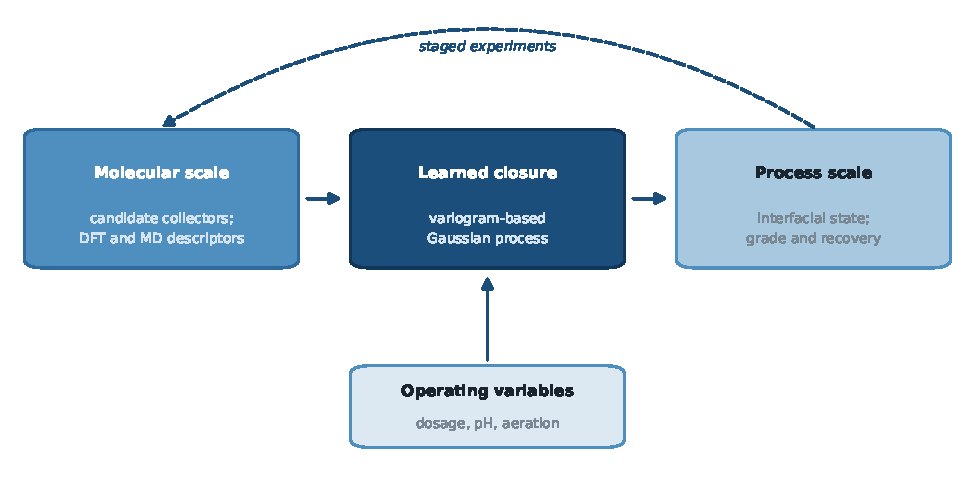
\includegraphics[width=0.93\textwidth]{fig1_loops.pdf}
\caption{The molecular scale and the process scale, joined by a single learned closure. The descriptors and the plant variables enter the same covariance model, and the experimental program closes the loop.}
\label{fig:loops}
\end{figure}

\section{A surrogate over molecular descriptors}
The covariance model is retained and moved into descriptor space. Periodic DFT provides adsorption energies, adsorption geometries, charge redistribution and frontier-orbital descriptors for a family of collectors on the mineral surface, while explicit-water MD resolves the water-mediated contribution, including hydration density, molecular orientation and radial distribution functions. Together these define a descriptor vector $\mathbf{d}$, and the closure is written
\begin{equation}
\bigl(\mathbf{d},\;\mathbf{x}_{\mathrm{op}}\bigr)\;\longrightarrow\;\text{interfacial state}\;\longrightarrow\;k\;\longrightarrow\;\text{grade and recovery},
\label{eq:closure}
\end{equation}
so that the descriptors constrain the interfacial state while the pre-fitted froth diagnostics carry the hydrodynamic part. Because the posterior is probabilistic, the inversion functions as a design tool rather than a lookup table: it ranks candidate molecules with an uncertainty interval on the selectivity--recovery trade-off, and identifies the region of descriptor space in which the predicted response is high but the posterior variance remains large (Fig.~\ref{fig:surrogate}).

The decisive question is whether the descriptors improve prediction, generalization and interpretability when added to a model that already contains the operating variables and the froth diagnostics, or whether a fit of the same data performs as well without them. This is answerable by ablation, removing each constraint in turn and reporting where it repays its cost.

\begin{figure}[!htbp]
\centering
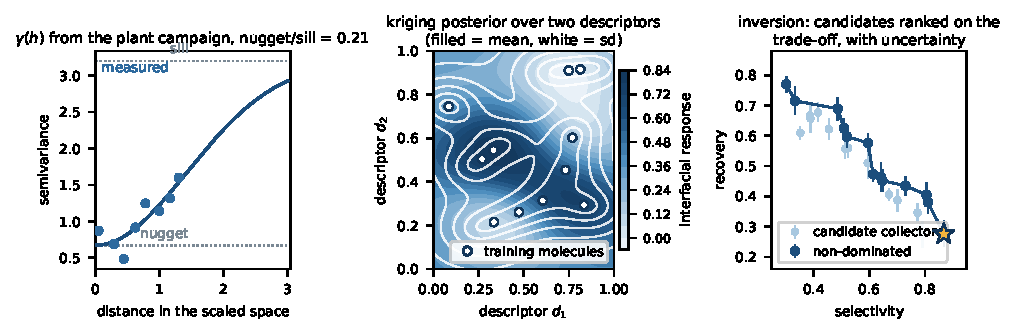
\includegraphics[width=\textwidth]{fig2_surrogate.pdf}
\caption{(a) The variogram recovered from the plant campaign, whose nugget is the finite reproducibility of a flotation test and whose ratio to the sill is 0.21. (b) A worked kriging posterior over two molecular descriptors. (c) The inversion that follows: candidates ranked on the selectivity--recovery trade-off, with intervals.}
\label{fig:surrogate}
\end{figure}

\section{Validation designed in rather than assumed}
The experimental program is planned before any model is fitted. A staged sequence --- screening, factorial design, response-surface refinement, then reserved tests --- generates the data, with replicates across days to separate real effects from day-to-day drift (Fig.~\ref{fig:program}). A block of conditions is reserved from the outset and never enters model development. The framework is judged on those conditions rather than on random train--test splits, since a random split of a designed campaign is not evidence that a ranking transfers to a condition the plant has not run. The reserved block also tests the practical claim: whether the framework orders a small external set of candidates, with intervals, in a sequence that the subsequent experiments confirm.

\begin{figure}[!htbp]
\centering
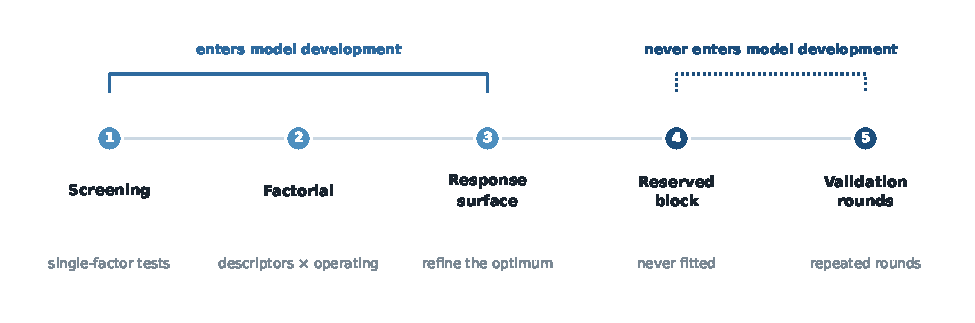
\includegraphics[width=\textwidth]{fig3_program.pdf}
\caption{Staged experimental program. Stages 1--3 build the model; the reserved block and the validation rounds never enter model development, so the ranking is judged on conditions the model has not seen.}
\label{fig:program}
\end{figure}

\section{What the framework would deliver}
The framework would deliver a chain from descriptor to performance in which each link is tested against an independent measurement, so that a failure is traced to one link rather than attributed to the approach as a whole. The same model yields a ranking of candidate collectors with uncertainty intervals, addressed to an experimental program rather than to a plant. The ablations establish which of the added constraints is worth its cost. The mineral--collector system is chosen for industrial relevance and analytical tractability, so the framework does not depend on a single ore source.

Mineral-X's interest in AI-driven reagent discovery, and in quantifying the uncertainty of a recommendation rather than only issuing it, makes this a natural setting for the idea. I have worked in both halves separately --- DFT and MD at mineral--water interfaces, and the geostatistical workflow applied to my own plant data --- and this note is how I would join them.

\end{document}
